\section{熊猫走钢丝}
\markboth{21. 熊猫走钢丝}{21. 熊猫走钢丝}

\noindent
\begin{minipage}[c]{0.41\textwidth}
  \centering
  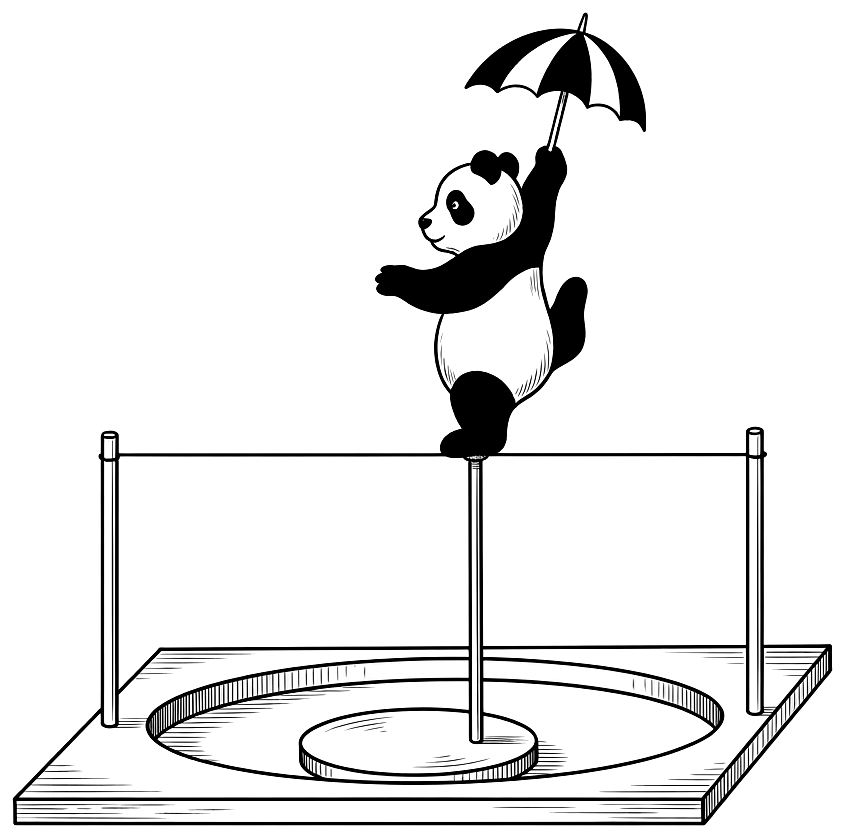
\includegraphics[width=\linewidth]{fig_021_1.png}
  \captionof*{figure}{图\ 21.1}
\end{minipage}\hfill
\begin{minipage}[c]{0.56\textwidth}
  \setlength{\parindent}{2em}\indent
  图 21.1 所画的场面，并不是马戏团表演镜头的真实写照，而只是根据数学原理设计的一个小玩具。玩具的底座上有一个圆洞，洞内有一块圆板，熊猫的模型通过细杆连接在圆板边缘上。把圆板沿圆洞边缘滚动（注意不要有滑动），就会看到细杆上端的熊猫一边沿钢丝滑动，一边还转动着肥胖的身体，非常有趣。
\end{minipage}

如果自己动手做一个这样的玩具，必须注意两个关键：第一，圆洞的直径要正好等于圆板直径的 $2$ 倍；第二，牵钢丝的两根柱子竖立在底座上的位置，应该位于圆洞的一条直径的延长线上。换句话说，钢丝在底座平面内的正射影应该是圆洞的一条直径。这个玩具的基本原理，就是下面的轨迹定理：

当半径为 $r$ 的动圆 $C$ 在半径为 $2r$ 的定圆 $O$ 内无滑动地滚动时，动圆圆周上一点 $M$ 的轨迹是圆 $O$ 的一条直径。

\noindent
\begin{minipage}[c]{0.50\textwidth}
  \setlength{\parindent}{2em}\indent
  现在证明上述事实。如图 21.2，取 $O$ 为坐标原点，并且选取 $x$ 轴，使得动圆的圆心落在 $x$ 轴正半轴上时，动圆 $C$ 上的 $M$ 点到 $O$ 的距离最远，即这时 $M(x, y)$ 将落在圆 $O$ 与 $x$ 轴正半轴的交点 $A$ 处。设动圆 $C$ 继续滚动到图中实线所示位置，这时的圆心为 $C(a, b)$，切点为 $B$，$\angle AOB=\theta$，则
\end{minipage}\hfill
\begin{minipage}[c]{0.47\textwidth}
  \centering
  \begin{tikzpicture}[scale=0.68, >=Stealth, line cap=round, line join=round]
    \def\r{1.0}
    \def\th{52}
    \coordinate (O) at (0,0);
    \coordinate (G) at (-2*\r, 0);
    \coordinate (A) at (2*\r, 0);
    \coordinate (B) at ({2*\r*cos(\th)}, {2*\r*sin(\th)});
    \coordinate (C) at ({\r*cos(\th)}, {\r*sin(\th)});
    \coordinate (M) at ({2*\r*cos(\th)}, 0);

    % 坐标轴
    \draw[->] (-2.28, 0) -- (2.60, 0) node[below, font=\footnotesize] {$x$};
    \draw[->] (0, -2.25) -- (0, 2.32) node[left, font=\footnotesize] {$y$};

    % 定圆 O、初始位置虚线圆、动圆 C
    \draw[thick] (O) circle (2*\r);
    \draw[dashed] (\r, 0) circle (\r);
    \draw[thick, curveblue] (C) circle (\r);

    % 线段 OB, CM 及延长线
    \draw (O) -- (B);
    \draw (C) -- (M);
    \draw[thin, dashed] (M) -- ++({-\th}:0.62);

    % 角 theta, phi, -theta
    \draw (0.40, 0) arc (0:\th:0.40);
    \node[font=\scriptsize] at ({0.56*cos(0.5*\th)}, {0.56*sin(0.5*\th)}) {$\theta$};

    \draw ($(C) + (\th:0.28)$) arc (\th:{-\th}:0.28);
    \node[font=\scriptsize] at ($(C) + (0.44, 0.05)$) {$\phi$};

    \draw ($(M) + (0:0.26)$) arc (0:{-\th}:0.26);
    \node[font=\scriptsize, fill=white, inner sep=0.5pt] at ($(M) + (-26:0.50)$) {$-\theta$};

    % 关键点与标签
    \fill (O) circle (1.3pt) node[below left, font=\footnotesize] {$O$};
    \fill (G) circle (1.3pt) node[below left, font=\footnotesize] {$G$};
    \fill (A) circle (1.3pt) node[below right=-1pt, font=\footnotesize] {$A$};
    \fill (B) circle (1.3pt) node[above right, font=\footnotesize] {$B$};
    \fill (C) circle (1.3pt) node[above left=-1pt, font=\footnotesize] {$C$};
    \fill (M) circle (1.4pt) node[below left=-1pt, font=\footnotesize] {$M$};
  \end{tikzpicture}
  \captionof*{figure}{图\ 21.2}
\end{minipage}
\[
  a = r\cos\theta,\quad b = r\sin\theta.
\]

又因为滚动时没有滑动，所以小圆的 $\arc{BM}$ 与大圆的 $\arc{BA}$ 长度相等。所以，如果记 $\angle BCM=\phi$，就有
\begin{align*}
  r\phi &= (2r)\cdot\theta, \\
  \therefore\quad \phi &= 2\theta.
\end{align*}

另一方面，$\angle COM = \angle CMO = \frac{1}{2}\phi = \theta$，所以 $M$ 点必落在 $x$ 轴上，且 $\overrightarrow{CM}$ 的幅角为 $-\theta$，由 $\overrightarrow{OM} = \overrightarrow{OC} + \overrightarrow{CM}$ 得
\begin{align*}
  (x, y) &= (r\cos\theta,\, r\sin\theta) + (r\cos(-\theta),\, r\sin(-\theta)) \\
         &= (2r\cos\theta,\, 0).
\end{align*}
这样就证明了点 $M(x, y)$ 的轨迹是 $x$ 轴上的线段 $-2r\leqslant x\leqslant 2r$，即定圆 $O$ 的直径 $GA$。
